\newpage
\section{Funktionen}

Eine Funktion ist eine Formel mit der man sich für jeden beliebigen $x$ Wert in einem Koordinatensytem einen entsprechenden $y$ Wert errechnen kann.\\
Eine Funktion weist einem unabhängigen Wert ($x$) genau einen abhängigen Wert ($y$) zu.\\

\hfill \break
Thermologie:\\
\begin{itemize}
    \item Ein Beispiel für einen Funktionsterm ist: $f(x) = 5x+10$
    \item Bei der Funktionen: $f(x) = 5x+10$ bezeichnet $x$ das Funktionsargument,
\end{itemize}

\hfill \break
die Funktion $y=2x-1$ kann als Wertetabelle...:\\
\fboxrule=0.8pt \fcolorbox{lightgray}{lightgray}{%
    \begin{tabular}{c|c}
        $x$ & $y$ \\
        \hline
        0   & -1  \\
        1   & 1   \\
        2   & 3   \\
        3   & 5   \\
        4   & 7   \\
    \end{tabular}}\\

\hfill \break
...und graphisch dargestellt erden:\\
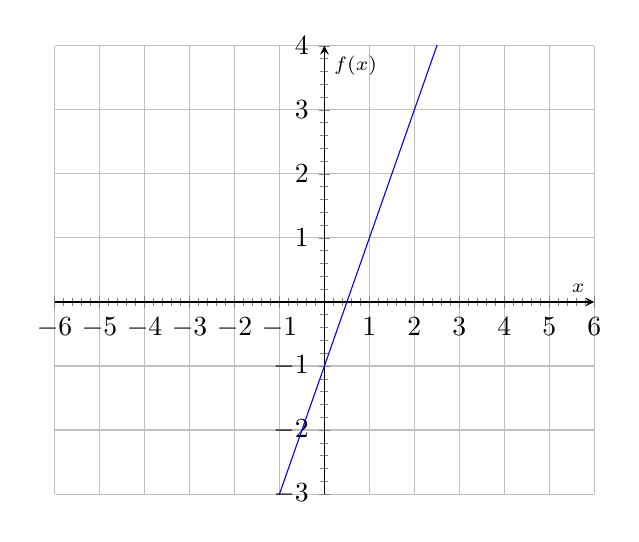
\begin{tikzpicture}[scale=1.0]
    \begin{axis}%
        [
            grid=major,
            xtick={-7,-6,...,7},
            minor x tick num=4, % 4 minor ticks => 5 subintervals
            xmin=-6,
            xmax=6,
            xlabel={\scriptsize $x$},
            axis x line=middle,
            ytick={-5,-4,...,5},
            minor y tick num=4,  % 4 minor ticks => 5 subintervals
            ymin=-3,
            ymax=4,
            ylabel={\scriptsize $f(x)$},
            axis y line=middle,
            no markers,
            samples=100,
            domain=-6:6,
        ]
        \addplot (x,{2*x-1});
    \end{axis}
\end{tikzpicture}

\break
\newpage
\subsection{Zusammenfassung aller Funtionstypen}

\begin{enumerate}
    \item Lineare Funktion: $f(x)=mx+n$ \begin{itemize}
              \item Definitionsbereich: $x\in\mathbb{R}$
              \item Wertebereich: $y\in\mathbb{R}$
              \item Nullstelle: $x_0=-\frac{n}{m}$
              \item streng monoton steigend
          \end{itemize}
    \item Quadratische Funktion: $f(x)=x^2+px+q$ \begin{itemize}
              \item Definitionsbereich: $x\in\mathbb{R}$
              \item Wertebereich: $x\in\mathbb{R},\geq-\frac{p^2}{4}+4$
              \item Nullstelle: $x_{1,2}=+\frac{p}{2} \pm \sqrt{\binom{p}{2}^2-q}$
              \item streng monoton steigend für $x \geq -\frac{p}{2}$
              \item streng monoton fallend für $x \leq -\frac{p}{2}$
          \end{itemize}
    \item Quadratische Funktion: $f(x)=ax^2+e$ \begin{itemize}
              \item Definitionsbereich: $x\in\mathbb{R}$
              \item Wertebereich: $y\in\mathbb{R},y\leq e$
              \item Nullstelle: $x_{1,2} = \pm \sqrt{-\frac{e}{a}}$
              \item streng monoton steigend für $x<0$
              \item streng monoton fallend für $x>0$
          \end{itemize}
    \item Wurzelfunktion: $f(x)=\sqrt{x}$\begin{itemize}
              \item Definitionsbereich: $x\in\mathbb{R},y\geq 0$
              \item Wertebereich: $y\in\mathbb{R},y\geq 0$
              \item Nullstelle: $x_0=0$
              \item streng monoton steigend
          \end{itemize}
    \item Potenzfunktion: $f(x)=x^n$\begin{itemize}
              \item Definitionsbereich: $x\in\mathbb{R},y\neq 0$
              \item Wertebereich: $y\in\mathbb{R},y\neq 0$
              \item Nullstelle: Nicht vorhanden
              \item streng monoton fallend für $x \neq 0$
          \end{itemize}
    \item Sinusfunktion: $f(x=sin(x))$\begin{itemize}
              \item Definitionsbereich: $x\in\mathbb{R}$
              \item Wertebereich: $y\in\mathbb{R},-1 \leq y \leq 1$
              \item Nullstelle: $x_k=k * \pi,k \in \mathbb{Z}$
              \item streng monoton steigend für $-\frac{\pi}{2}\leq x \leq \frac{\pi}{2}$
              \item streng monoton fallend für $\frac{\pi}{2}\leq x \leq \frac{3\pi}{2}$
          \end{itemize}
    \item Exponential-funktion: $f(x)=a*b^x$\begin{itemize}
              \item Definitionsbereich: $x\in\mathbb{R}$
              \item Wertebereich: $y\in\mathbb{R},y > 0$
              \item Nullstelle: Nicht vorhanden
              \item streng monoton fallend für
          \end{itemize}
    \item Logarithmus-funktion: $f(x)=log_b(x)$\begin{itemize}
              \item Definitionsbereich: $x\in\mathbb{R},x > 0$
              \item Wertebereich: $y\in\mathbb{R}$
              \item Nullstelle: $x_0=1$
              \item streng monoton steigend für
          \end{itemize}
\end{enumerate}


\break
\newpage
\subsection{Steigung}

Die Steigung ist das Verhältnis von $x$ zu $y$.\\
Am Beispiel von $y = -2x+5$ bei einem Schritt von $+1$ nach $x$ ändert sich $y$ um $-2$ daher ist die Steigung $\frac{-2}{1}$.


\hfill \break
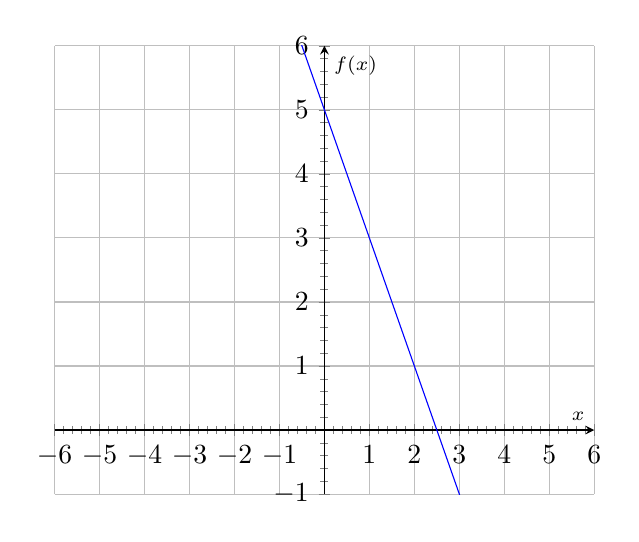
\begin{tikzpicture}[scale=1.0]
    \begin{axis}%
        [
            grid=major,
            xtick={-7,-6,...,7},
            minor x tick num=4, % 4 minor ticks => 5 subintervals
            xmin=-6,
            xmax=6,
            xlabel={\scriptsize $x$},
            axis x line=middle,
            ytick={-5,-4,...,6},
            minor y tick num=4,  % 4 minor ticks => 5 subintervals
            ymin=-1,
            ymax=6,
            ylabel={\scriptsize $f(x)$},
            axis y line=middle,
            no markers,
            samples=100,
            domain=-6:6,
        ]
        \addplot (x,{-2*x+5});
        \slopeTriangle{0.8}{0.1}{0.5}{1}{blue}; % USE OF MACRO.
    \end{axis}
\end{tikzpicture}
\break
\newpage
\subsection{Einteilung der Funktionen}

Funktionen werden in verschiedenen Arten unterschieden:\\
\begin{enumerate}
    \item Funktion 1.Grades (Lineare Funktion):\textcolor{red}{$f(x)=a+x^1+d$}
    \item Funktion 2.Grades (Quadratische Funktion):\textcolor{blue}{$f(x)=ax^2+bx^1+d$}
    \item Funktion 3.Grades (Kubische Funktion):\textcolor{violet}{$f(x)=ax^3+bx^2+cx^1+d$}
\end{enumerate}


\hfill \break
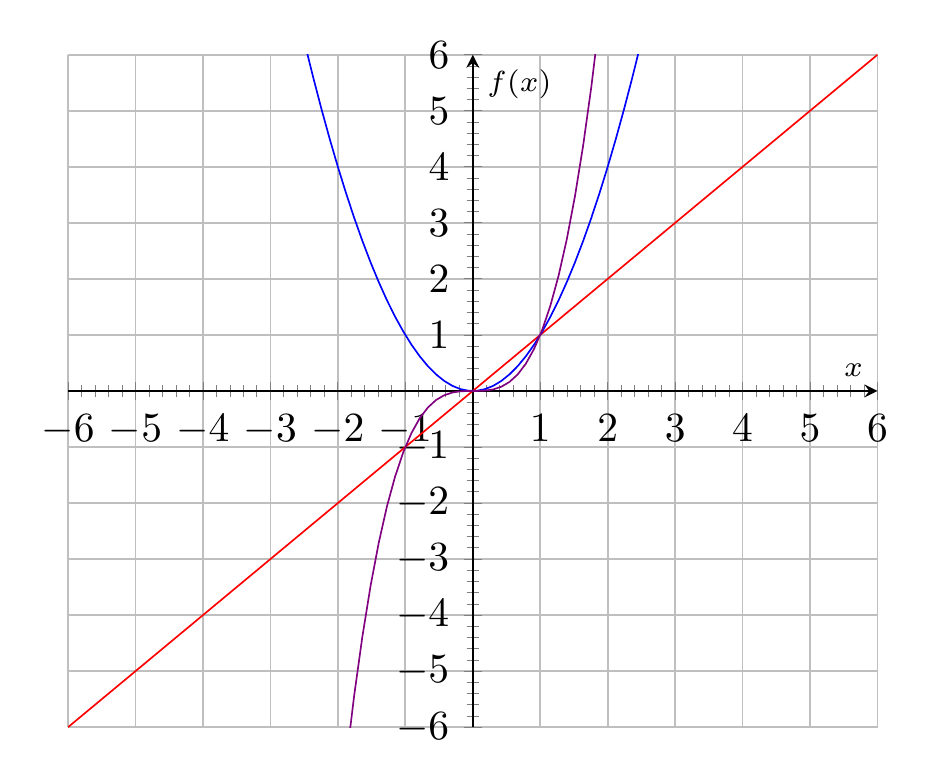
\begin{tikzpicture}[scale=1.5]
    \begin{axis}%
        [
            grid=major,
            xtick={-7,-6,...,7},
            minor x tick num=4, % 4 minor ticks => 5 subintervals
            xmin=-6,
            xmax=6,
            xlabel={\scriptsize $x$},
            axis x line=middle,
            ytick={-6,-5,...,7},
            minor y tick num=4,  % 4 minor ticks => 5 subintervals
            ymin=-6,
            ymax=6,
            ylabel={\scriptsize $f(x)$},
            axis y line=middle,
            no markers,
            samples=100,
            domain=-6:6,
        ]
        \addplot[red] (x,{x});
        \addplot[blue] (x,{x*x});
        \addplot[violet] (x,{x*x*x});
    \end{axis}
\end{tikzpicture}
\break
\newpage
\subsection{Lineare Funktionen}

Die Grundform einer jeden linearen Funktion ist $y=k*x+d$.
Wobei...

\begin{itemize}
    \item ... $y$ das das Resultat der Gleichung ist
    \item ... $k$ die Steigung der linearen Funktion ist
    \item ... $x$ die Variable ist
    \item ... $d$ der Abstand zur $x$ Achse ist
\end{itemize}

\hfill \break
Wenn das $k$ der Gleichung...
\begin{itemize}
    \item $>0$ ist wird die Gerade steigend z.B. \textcolor{red}{$y=3x+1$}
    \item $<0$ ist wird die Gerade fallend z.B. \textcolor{green}{$y=-3x+1$}
    \item $=0$ ist wird die Gerade waagrecht z.B. \textcolor{blue}{$y=1$}
\end{itemize}

\hfill \break
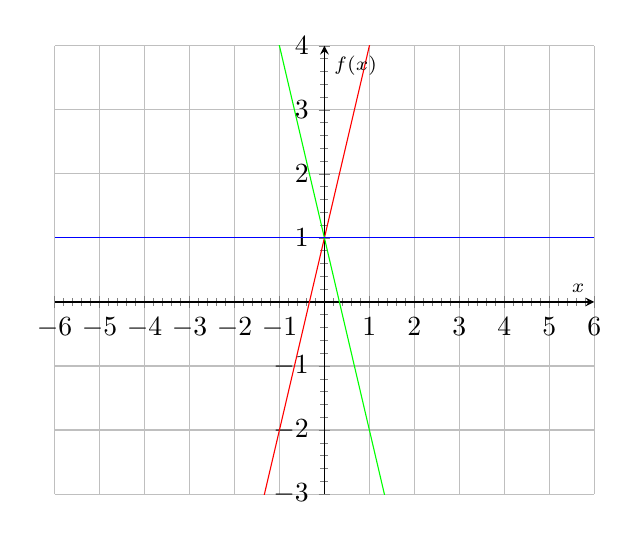
\begin{tikzpicture}[scale=1.0]
    \begin{axis}%
        [
            grid=major,
            xtick={-7,-6,...,7},
            minor x tick num=4, % 4 minor ticks => 5 subintervals
            xmin=-6,
            xmax=6,
            xlabel={\scriptsize $x$},
            axis x line=middle,
            ytick={-5,-4,...,5},
            minor y tick num=4,  % 4 minor ticks => 5 subintervals
            ymin=-3,
            ymax=4,
            ylabel={\scriptsize $f(x)$},
            axis y line=middle,
            no markers,
            samples=100,
            domain=-6:6,
        ]
        \addplot[red] (x,{3*x+1});
        \addplot[green] (x,{-3*x+1});
        \addplot[blue] (x,{1});
    \end{axis}
\end{tikzpicture}
\break
\newpage
\subsection{Lineare Funktionen mit 2 Variablen}

Jede lineare Gleichung lässt sich auf eine Faktorgleichung der Form $y=kx+d$ umformen.
$$ax+by = c$$
$$\downarrow$$
$$y=\frac{c-ax}{b}$$

\hfill \break
Example:\\
\fboxrule=0.8pt \fcolorbox{black}{lightgray}{%
    \begin{tabular}[t]{@{}l@{}}
        $x+y=5$ /-x \\
        $y=5-x$     \\
        $y=-x+5$    \\
        $y=-1x+5$   \\
    \end{tabular}}
\begin{itemize}
    \item $d=5$
    \item $k=-1$
\end{itemize}

\hfill \break
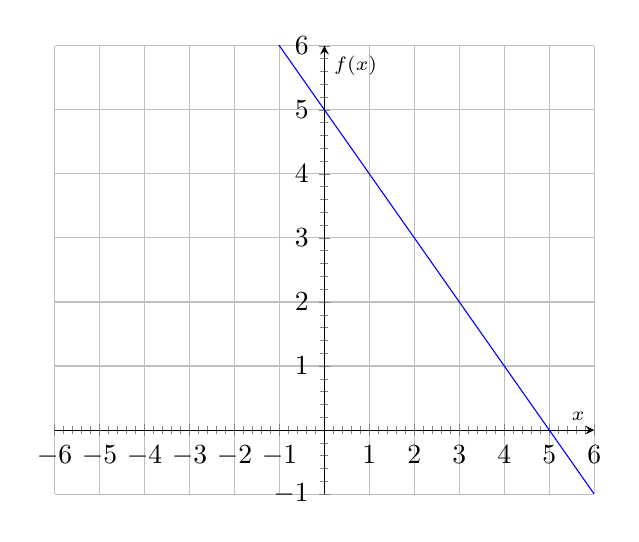
\begin{tikzpicture}[scale=1.0]
    \begin{axis}%
        [
            grid=major,
            xtick={-7,-6,...,7},
            minor x tick num=4, % 4 minor ticks => 5 subintervals
            xmin=-6,
            xmax=6,
            xlabel={\scriptsize $x$},
            axis x line=middle,
            ytick={-5,-4,...,6},
            minor y tick num=4,  % 4 minor ticks => 5 subintervals
            ymin=-1,
            ymax=6,
            ylabel={\scriptsize $f(x)$},
            axis y line=middle,
            no markers,
            samples=100,
            domain=-6:6,
        ]
        \addplot (x,{-1*x+5});
    \end{axis}
\end{tikzpicture}

\hfill \break
Lösungsverfahren:
\begin{itemize}
    \item Graphisch
    \item Rechnerisches Gleichsetzungsverfahren
    \item Rechnerisches Einsetzungsverfahren
    \item Rechnerisches Eliminationsverfahren
\end{itemize}

\break
\newpage
\subsubsection{Gleichsetzungsverfahren}

Beim Gleichsetzungsverfahren werden beide Terme Gleichgesetzt.

\hfill \break
Example:\\
\fboxrule=0.8pt \fcolorbox{black}{lightgray}{%
    \begin{tabular}[t]{@{}l@{}}
        (1):$y=x+1 $ / $y=2$   \\
        (2):$y=-2x+4 $ / $y=2$ \\
        \\
        \\
        $y_1 = y_2$            \\
        $x+1 = -2x+4$ /+2x     \\
        $3x+1 = 4$ /-1         \\
        $3x = 3$ / /3          \\
        $x = 1$                \\
    \end{tabular}}

$$L=\{1,2\}$$
\break
\subsubsection{Einsezuungsverfahren}

Beim Einsezuungsverfahren wird ein Term in den anderen eingesetzt.

\hfill \break
Example:\\
\fboxrule=0.8pt \fcolorbox{black}{lightgray}{%
    \begin{tabular}[t]{@{}l@{}}
        (1):$y=x+1$                                  \\
        (2):$+2x+y=4$ / $x+1$ wird in $y$ eingesetzt \\
        \\
        \\
        $+2x+x+1 = 4$                                \\
        $3x+1 = 4$ / -1                              \\
        $3x = 3$ / /3                                \\
        $x = 1$                                      \\
    \end{tabular}}

$$L=\{1,2\}$$
\break
\newpage
\subsubsection{Eliminationsverfahren}

Beim Eliminationsverfahren wird ein Teil des ersten Termes vom zweiten Term subtrahiert.

\hfill \break
Example:\\
\fboxrule=0.8pt \fcolorbox{black}{lightgray}{%
    \begin{tabular}[t]{@{}l@{}}
        (1):$y=x+1$ /$y$ wird elemeniert   \\
        (2):$y=-2x+4$ /$y$ wird elemeniert \\
        \\
        \\
        $0=x-(-2x)+1-4$                    \\
        $0=x+2x-3$                         \\
        $3=3x$ / /3                        \\
        $1=x$                              \\
    \end{tabular}}

$$L=\{1,2\}$$

\hfill \break
Um $x$ elemenieren zu können muss man zuerst bei beide Gleichungen die selbe Anzahl an $x$ erzeugen.

\hfill \break
Example:\\
\fboxrule=0.8pt \fcolorbox{black}{lightgray}{%
    \begin{tabular}[t]{@{}l@{}}
        (1):$4x + y = 16$          \\
        (2):$4x - 2y  = - 8 $ / /2 \\
        (2):$2x - y  = - 4$        \\
        \\
        \\
        $4x+y=16$                  \\
        $2x-y=-4$                  \\
        $6x=12$                    \\
        $x=2$                      \\
        \\
        \\
        In Ursprungsform Einsetzen \\
        $4*2+y=16$                 \\
        $8+y=16$ / -8              \\
        $y=8$                      \\
    \end{tabular}}

$$L=\{2,8\}$$
\newpage
\subsubsection{Sonderfälle}

\hfill \break
Example 1.Sonderfall:\\
\fboxrule=0.8pt \fcolorbox{black}{lightgray}{%
    \begin{tabular}[t]{@{}l@{}}
        (1):$3x+2y=4$ / *2 \\
        (2):$-6x-4y=-8$    \\
        (1):$6x+4y=8$      \\
        \\
        \\
        $0+0 = 0$          \\
        $0 = 0$            \\
    \end{tabular}}\\

\hfill \break
Example 2.Sonderfall:\\
\fboxrule=0.8pt \fcolorbox{black}{lightgray}{%
    \begin{tabular}[t]{@{}l@{}}
        (1):$3x+2y=4$ / *3 \\
        (2):$9x+6y=10$     \\
        (1):$9x+6y=12$     \\
        \\
        \\
        $0+0 = 2$          \\
        $0 = 2$ / $f.A$    \\
    \end{tabular}}\\
\break
\newpage
\subsection{Funktionsgleichung bestimmen}

Es gibt zwei Arten der Bestimmung der Funktionsgleichung:\\

\hfill \break
\fboxrule=0.8pt \fcolorbox{black}{lightgray}{%
    \begin{tabular}[t]{@{}l@{}}
        $A(1/8)$  \\
        $B(-4/3)$ \\
        \hline
        $y=kx+d$
    \end{tabular}}\\

\hfill \break
1.Graphisch:\\
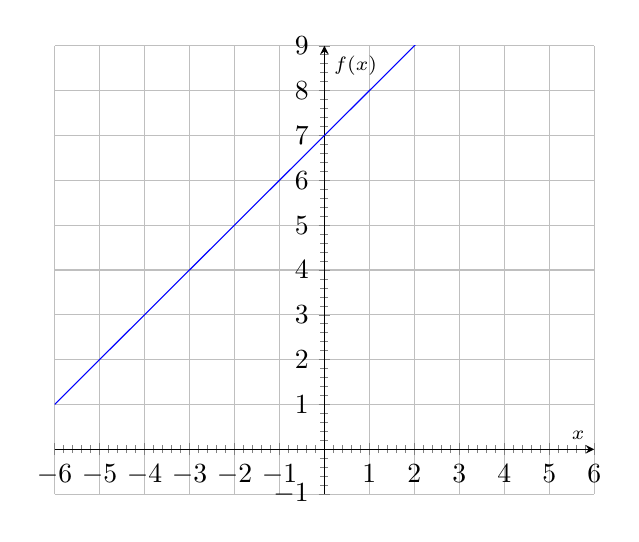
\begin{tikzpicture}[scale=1.0]
    \begin{axis}%
        [
            grid=major,
            xtick={-7,-6,...,7},
            minor x tick num=4, % 4 minor ticks => 5 subintervals
            xmin=-6,
            xmax=6,
            xlabel={\scriptsize $x$},
            axis x line=middle,
            ytick={-5,-4,...,9},
            minor y tick num=4,  % 4 minor ticks => 5 subintervals
            ymin=-1,
            ymax=9,
            ylabel={\scriptsize $f(x)$},
            axis y line=middle,
            no markers,
            samples=100,
            domain=-6:6,
        ]
        \addplot[blue] (x,{x+7});
    \end{axis}
\end{tikzpicture}

\hfill \break
\fboxrule=0.8pt \fcolorbox{black}{lightgray}{%
    \begin{tabular}[t]{@{}l@{}}
            $d=7$ \\
            $k=1$ \\
            \hline
            $y=kx+d$
        \end{tabular}}\\

\hfill \break
2.Rechnerisch:\\
\fboxrule=0.8pt \fcolorbox{black}{lightgray}{%
    \begin{tabular}[t]{@{}l@{}}
            (1):$8=1k+d$                                            \\
            (2):$\textcolor{blue}{3=-4k+d}$                         \\
            (1):$d=-k+8$                                            \\
            $3=-4k-k+8$ / ermittelt durch das Eliminationsverfahren \\
            $k=\textcolor{red}{1}$                                  \\
            \\
            $\textcolor{blue}{3=-4*\textcolor{red}{1}+d}$           \\
            $d=7$                                                   \\
        \end{tabular}}\\
\break
\newpage
\subsection{Kostenfunktion}

Die Grundform der Kostenfunktion ist $K(x)=k*x+F$.
Wobei...
\begin{itemize}
    \item ... $K(x)$ ist das Resultat der Gleichung ist also die Kosten.
    \item ... $k$ die Kosten pro Stück darstellt
    \item ... $x$ die Menge ist
    \item ... $F$ die Fixkosten darstellt
\end{itemize}

\hfill \break
Die Grundform der Erlösfunktion ist $E(x)=p*x$.
Wobei...
\begin{itemize}
    \item ... $E(x)$ ist das Resultat der Gleichung ist also der Erlös des Verkaufs
    \item ... $p$ der Verkaufspreis
    \item ... $x$ die Verkaufsmenge ist
\end{itemize}

\hfill \break
Die Grundform der Gewinnfunktion ist $G(x)=E(x)-K(x)$.
Wobei $G(x)$ der Gewinn ist.

\hfill \break
Example:\\
Die Fixkosten eines Betriebes betragen 140000€ pro Monat, die Produktionskosten 4€ pro Stück. Ein Stück wird zu 8€
verkauft.
Wie viel Stück müssen verkauft werden, damit ein Gewinn von mindestens 1000 000€ erzielt wird?:\\
\fboxrule=0.8pt \fcolorbox{black}{lightgray}{%
    \begin{tabular}[t]{@{}l@{}}
        $K(x)=4x+140000$             \\
        $E(x)=8x$                    \\
        $G(x)=E(x)-K(x)$             \\
        \hline
        $1000000=8x-(4x+140000)$     \\
        $1000000=8x-4x-140000$       \\
        $1000000=4x-140000$ /+140000 \\
        $1140000=4x$ / /4            \\
        $x=285000$                   \\
    \end{tabular}}
\break
\newpage
\subsection{Normale/Paralelle Lineare Funktionen}

Die zu einer Geraden normale Gerade erhält man durch den negativen Kehrwert: $K\bot = -\frac{1}{k}$

\hfill \break
Example normale Funktionenen:\\
\fboxrule=0.8pt \fcolorbox{black}{lightgray}{%
    \begin{tabular}[t]{@{}l@{}}
        $\textcolor{red}{y=\frac{3}{4}x}$      \\
        $\textcolor{green}{y_n=-\frac{4}{3}x}$ \\
    \end{tabular}}

\hfill \break
Example paralelle Funktionenen:\\
\fboxrule=0.8pt \fcolorbox{black}{lightgray}{%
    \begin{tabular}[t]{@{}l@{}}
        $\textcolor{blue}{y = 3x-1}$   \\
        $\textcolor{violet}{y = 3x+3}$ \\
    \end{tabular}}

\hfill \break
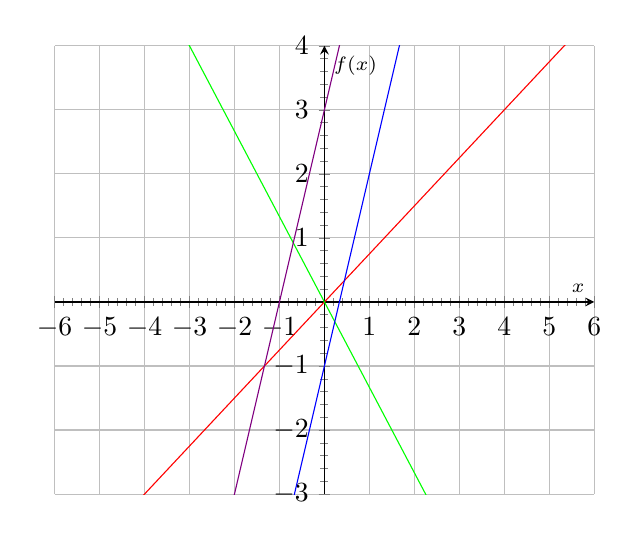
\begin{tikzpicture}[scale=1.0]
    \begin{axis}%
        [
            grid=major,
            xtick={-7,-6,...,7},
            minor x tick num=4, % 4 minor ticks => 5 subintervals
            xmin=-6,
            xmax=6,
            xlabel={\scriptsize $x$},
            axis x line=middle,
            ytick={-5,-4,...,5},
            minor y tick num=4,  % 4 minor ticks => 5 subintervals
            ymin=-3,
            ymax=4,
            ylabel={\scriptsize $f(x)$},
            axis y line=middle,
            no markers,
            samples=100,
            domain=-6:6,
        ]
        \addplot[red] (x,{(3/4)*x});
        \addplot[green] (x,{-(4/3)*x});
        \addplot[blue] (x,{3*x-1});
        \addplot[violet] (x,{3*x+3});
    \end{axis}
\end{tikzpicture}

\hfill \break
Example normale Funktionenen:\\
\fboxrule=0.8pt \fcolorbox{black}{lightgray}{%
    \begin{tabular}[t]{@{}l@{}}
        $y_1 = \frac{2}{3}x \bot y_1=-\frac{3}{2}x$ \\
        \\
        $y_2 = 2x \bot y_2=+\frac{1}{2}x$           \\
        \\
        $y_3 = -\frac{1}{3}x+1 \bot y_3=3x+1$       \\
    \end{tabular}}

\hfill \break
Example paralelle Funktionenen:\\
\fboxrule=0.8pt \fcolorbox{black}{lightgray}{%
    \begin{tabular}[t]{@{}l@{}}
        $y_1 = 3x-1 \| y_1 = 3x+1 $            \\
        \\
        $y_2 = 10x+101 \| y_2 = 10x-8 $        \\
        \\
        $y_3 = 5x+83 \| y_3 = 5x+\frac{1}{2} $ \\
    \end{tabular}}
\break
\newpage
\subsection{Funktionswerte}

\hfill \break
\subsubsection{steigen und sinken}

Es gibt verschieden Arten von Funktionen:\\
\begin{itemize}
    \item \textcolor{red}{Streng monoton steigend $f'(x)>0$}
    \item \textcolor{violet}{Konstant $f'(x)=0$}
    \item \textcolor{blue}{Streng monoton fallend $f'(x)<0$ }
\end{itemize}

\hfill \break

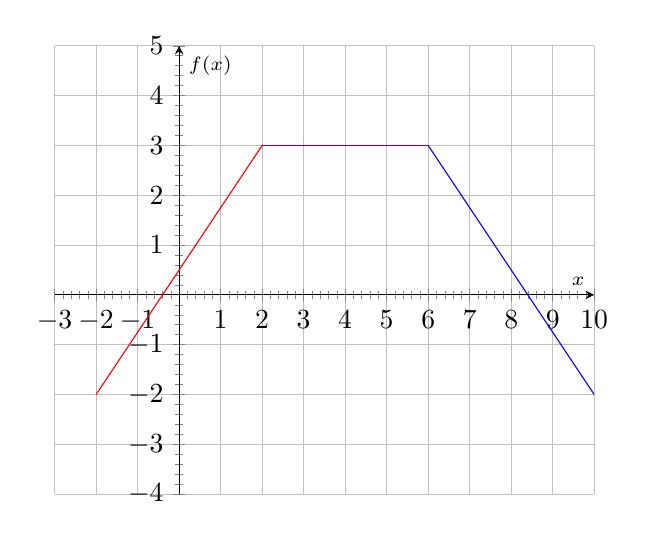
\begin{tikzpicture}[scale=1.0]
    \begin{axis}%
        [
            grid=major,
            xtick={-7,-6,...,11},
            minor x tick num=4, % 4 minor ticks => 5 subintervals
            xmin=-3,
            xmax=10,
            xlabel={\scriptsize $x$},
            axis x line=middle,
            ytick={-6,-5,...,6},
            minor y tick num=4,  % 4 minor ticks => 5 subintervals
            ymin=-4,
            ymax=5,
            ylabel={\scriptsize $f(x)$},
            axis y line=middle,
            no markers,
            samples=100,
            domain=-6:6,
        ]
        \draw[red] (-2,-2) -- (2,3);
        \draw[violet] (2,3) -- (6,3);
        \draw[blue] (6,3) -- (10,-2);
    \end{axis}
\end{tikzpicture}
\hfill \break
\newpage
\subsubsection{globale und lokale Extreme}

\begin{itemize}
    \item \textcolor{red}{${a,b}$ sind Randextreme}
    \item \textcolor{violet}{$x_1,x_2$ sind lokale Extreme}
\end{itemize}

\hfill \break
\begin{itemize}
    \item Globale Extrmes sind Extreme bezüglich des Gesammten Definitionsbereich.
    \item Lobale Extrmes sind Extreme bezüglich eines klienen Bereiches.
    \item Extremstellen haben wagrechte Tangenten mit der Steigung $0$
\end{itemize}

\hfill \break
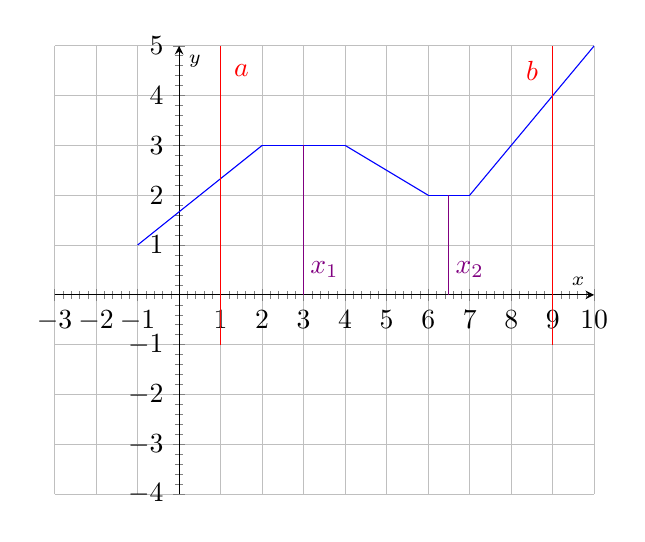
\begin{tikzpicture}[scale=1.0]
    \begin{axis}%
        [
            grid=major,
            xtick={-7,-6,...,11},
            minor x tick num=4, % 4 minor ticks => 5 subintervals
            xmin=-3,
            xmax=10,
            xlabel={\scriptsize $x$},
            axis x line=middle,
            ytick={-6,-5,...,6},
            minor y tick num=4,  % 4 minor ticks => 5 subintervals
            ymin=-4,
            ymax=5,
            ylabel={\scriptsize $y$},
            axis y line=middle,
            no markers,
            samples=100,
            domain=-6:6,
        ]
        \draw[blue] (-1,1) -- (2,3);
        \draw[blue] (2,3) -- (4,3);
        \draw[blue] (4,3) -- (6,2);
        \draw[blue] (6,2) -- (7,2);
        \draw[blue] (7,2) -- (10,5);
        \draw[red] (1,-1) -- (1,5);
        \draw[red] (9,-1) -- (9,5);
        \node[red] at (1.5,4.5) {$a$};
        \node[red] at (8.5,4.5) {$b$};

        \draw[violet] (3,0) -- (3,3);
        \draw[violet] (6.5,0) -- (6.5,2);
        \node[violet] at (3.5,0.5) {$x_1$};
        \node[violet] at (7,0.5) {$x_2$};
    \end{axis}
\end{tikzpicture}
\break
\newpage
\subsection{Quadratische Funktionen}

\begin{itemize}
    \item Die Grundform ist $y=a(x+b)^2+c$
    \item Faktorisierte Form ist $f(x)=a(x+x_1)*(x-x_2)$
    \item Scheitelpunktform oder Scheitelform ist $f(x)=a(x-d)^2+e$ mit Scheitel $S(d|e)$
\end{itemize}

\hfill \break
Veränderung der Normparabel:
\begin{itemize}
    \item Normparabel: \textcolor{black}{$x^2$}
    \item ist \textcolor{red}{$a<0$} wird die Funktion an der x Achse gespiegelt.
    \item ist \textcolor{blue}{$0<a<1$} wird die Funktion breiter bezihungsweise gestaucht.
    \item ist \textcolor{violet}{$a>1$} wird die Funktion steiler.
    \item ist \textcolor{cyan}{$x>0$} wird die Funktion nach oben verschoben.
    \item ist \textcolor{orange}{$x<0$} wird die Funktion nach oben verschoben.
    \item ist \textcolor{green}{$y<0$} wird die Funktion nach rechts verschoben.
    \item ist \textcolor{brown}{$y>0$} wird die Funktion nach links verschoben.
\end{itemize}

\hfill \break
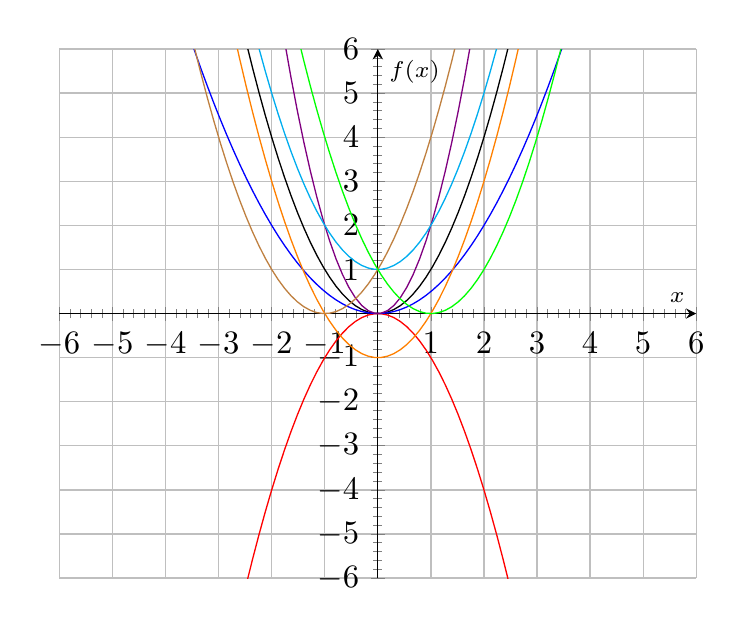
\begin{tikzpicture}[scale=1.18]
    \begin{axis}%
        [
            grid=major,
            xtick={-7,-6,...,7},
            minor x tick num=4, % 4 minor ticks => 5 subintervals
            xmin=-6,
            xmax=6,
            xlabel={\scriptsize $x$},
            axis x line=middle,
            ytick={-7,-6,...,7},
            minor y tick num=4,  % 4 minor ticks => 5 subintervals
            ymin=-6,
            ymax=6,
            ylabel={\scriptsize $f(x)$},
            axis y line=middle,
            no markers,
            samples=100,
            domain=-6:6,
        ]
        \addplot[black] (x,{x^2});
        \addplot[red] (x,{-1*x^2});
        \addplot[blue] (x,{0.5*x^2});
        \addplot[violet] (x,{2*x^2});
        \addplot[cyan] (x,{x^2+1});
        \addplot[orange] (x,{x^2-1});
        \addplot[brown] (x,{(x+1)^2});
        \addplot[green] (x,{(x-1)^2});
    \end{axis}
\end{tikzpicture}
\break
\newpage
\subsection{Nullstellenberechnung}

Nullstellen sind Stellen an denen eine Funktion die $x$ Achse schneidet. Dort ist der Funktionswert $0$.
Diese könne einfach mit der ABC-Formel gelöst werden in dem dei Faktoren eisetzt.\\

Example:\\
\fboxrule=0.8pt \fcolorbox{black}{lightgray}{%
    \begin{tabular}[t]{@{}l@{}}
        $f(x)=0$   \\
        $-x^2+4=0$ \\
        $x^2=4$    \\
        $x=\pm 2$  \\
    \end{tabular}}\\

Example:\\
\fboxrule=0.8pt \fcolorbox{black}{lightgray}{%
    \begin{tabular}[t]{@{}l@{}}
        $3x^2+6x=0$   \\
        $3x(x-2)$     \\
        $x=\pm 2$     \\
        $x=0$         \\
        $x=2$         \\
        $N_1 = (0,0)$ \\
        $N_2 = (2,0)$ \\
    \end{tabular}}\\

Example:\\
\fboxrule=0.8pt \fcolorbox{black}{lightgray}{%
    \begin{tabular}[t]{@{}l@{}}
        $f(x)=-x^2+7x=0$                               \\
        $\textcolor{red}{x}\textcolor{blue}{(-x+7)}=0$ \\
        $x_1= \textcolor{red}{0}$                      \\
        $x_2=\textcolor{blue}{7}$                      \\
    \end{tabular}}\\

Example:\\
\fboxrule=0.8pt \fcolorbox{black}{lightgray}{%
    \begin{tabular}[t]{@{}l@{}}
        $f(x)=x^2-4x+3=0$                                 \\
        $x^2-4x\textcolor{red}{+4}=-3\textcolor{red}{+4}$ \\
        $(x\textcolor{red}{-2})^2 = 1$                    \\
        $x-2= \pm \sqrt{1}$                               \\
        $x = 2 \pm 1$                                     \\
        $x_1 = 3$                                         \\
        $x_2 = 1$                                         \\
    \end{tabular}}\\

Rechnungsweg im Taschenrechner $TI-82STATS$:\\
\begin{itemize}
    \item $2nd$ calc zerro
    \item Cursor 1 neben die nullstellen links plazieren 
    \item Cursor 2 neben die nullstellen rechts plazieren
\end{itemize}
\break
\newpage
\subsection{Funktionen Aufstellen}

2.
Die nebenstehende Kurve veranschaulicht die Wurfparabel eines vom Punkt A
rückgespielten Tennisballs. Der Abschusspunkt liegt 6m vor dem Netz in Höhe
von 0,60m. Der Ball überfliegt das Netz in einer Höhe von 1,20m (B) und trifft
6,00m hinter dem Netz den Boden (C).\\

\begin{itemize}
    \item (a) Man berechne die Funktionsgleichung der Wurfparabel.
    \item (b) Welche Höhe erreicht der Ball 2m nachdem er das Netz passiert hat.
    \item (c) Wo hat der Ball eine Höhe von 80cm?
\end{itemize}

\hfill \break


Angegebene Punkte:
\begin{itemize}
    \item $A = (-6|0.6)$
    \item $A = (0|1.2)$
    \item $A = (0|0)$
\end{itemize}

\hfill \break

Eingesetzt in die Glichung $f(x)=a*x^2+b*x+c$:
\begin{enumerate}
    \item $0.6 = 36a-6b+c$
    \item $1.2 = 0a+0b+c$
    \item $0 = 36a+6b+c$
\end{enumerate}

\hfill \break

A:
$\left(\begin{array}{ccccc}
            36 & -6 & 1 & 0.6 \\
            0  & 0  & 1 & 1.2 \\
            36 & 6  & 1 & 0   \\
        \end{array}\right)$\\

\hfill \break

Ergebnis der Matrix Rechnung:
\begin{itemize}
    \item $a = -0.025$
    \item $b = -0.05$
    \item $c = 1.2$
\end{itemize}

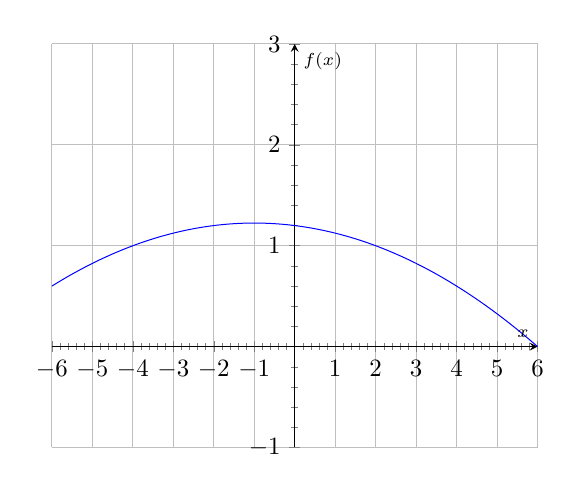
\begin{tikzpicture}[scale=0.9]
    \begin{axis}%
        [
            grid=major,
            xtick={-7,-6,...,7},
            minor x tick num=4, % 4 minor ticks => 5 subintervals
            xmin=-6,
            xmax=6,
            xlabel={\scriptsize $x$},
            axis x line=middle,
            ytick={-5,-4,...,3},
            minor y tick num=4,  % 4 minor ticks => 5 subintervals
            ymin=-1,
            ymax=3,
            ylabel={\scriptsize $f(x)$},
            axis y line=middle,
            no markers,
            samples=100,
            domain=-6:6,
        ]
        \addplot (x,{-0.025*x^2-0.05*x+1.2});
    \end{axis}
\end{tikzpicture}


\subsubsection{Lösung der Aufgabe A}
Die Funktionsgleichung wurden ermittelt in dem die Ergebnisse der Matrix in die Gleichung $f(x)=a*x^2+b*x+c$ Eingesetzt wurden.\\
Die Funktionsgleichung Lauted: $f(x)=-0.025x^2-0.05x+1.2$
\subsubsection{Lösung der Aufgabe B}
Bei dieser Aufgabe muss man den gewünschten Wert (in diesem Fall $2$) in die Funktionsgleichung die bei Beispiel $A$ errechnet wurde einsetzten.
Das Ergebnis lauted $1$
\subsubsection{Lösung der Aufgabe C}
Bei dieser Aufgabe werden die 80cm in Meter umgerechnet und als Ergebnis der Gleichung angegeben so, das $0.8 = -0.025x^2-0.05x+1.2$ entseht.
Danach muss die Gleichung durch eine Division durch $0.8$ noch auf die Form "0 = " gebracht werdendamit Man dei ABC-Formel anwenden kann.\\
die Ergebnisse lauten:
\begin{itemize}
    \item $x_1 = 3.12$
    \item $x_2 = 5.12$
\end{itemize}
\break
\newpage
\subsection{Exponentialfunktionen}


allgemeine Form: $y=a^x$
\begin{itemize}
    \item wenn $a>1$: Wachstum der Funktion
    \item wenn $0<a<1$: Zerfall der Funktion
\end{itemize}

\hfill \break
Eigenschaften:
\begin{itemize}
    \item alle Funktionen vom Typ $y=a^x$ haben den Punkt $P(0|1)$ gemein.
    \item alle Funktionen vom Typ $y=a^x$ gehen durch den Punkt $P(1|a)$, da $y=a^1 = a$.
    \item $y=a^x$ ist zu $y=a^{-x}$ symetrisch bezüglich der y Achse.
    \item die Funktion $y=a^x$ kann nie negativ werden also hat sie keine Nullstellen.
    \item Die x Achse ist eine Asymptote da die Funktion 0 niemals berührt.
\end{itemize}

\hfill \break
Die Wertetabellen und Grafik für \textcolor{red}{$y=2^x$} und \textcolor{blue}{$y=2^{-x}$}:\\

\hfill \break
\fboxrule=0.8pt \fcolorbox{lightgray}{lightgray}{%
    \begin{tabular}{c|c||c|c}
        \textcolor{red}{$x$} & $y$  & \textcolor{blue}{$x$} & $y$  \\
        \hline
        -2                   & 0.25 & -2                   & 4    \\
        -1                   & 0.5  & -1                   & 2    \\
        0                    & 1    & 0                    & 1    \\
        1                    & 2    & 1                    & 0.5  \\
        2                    & 4    & 2                    & 0.25 \\
    \end{tabular}}

\hfill \break
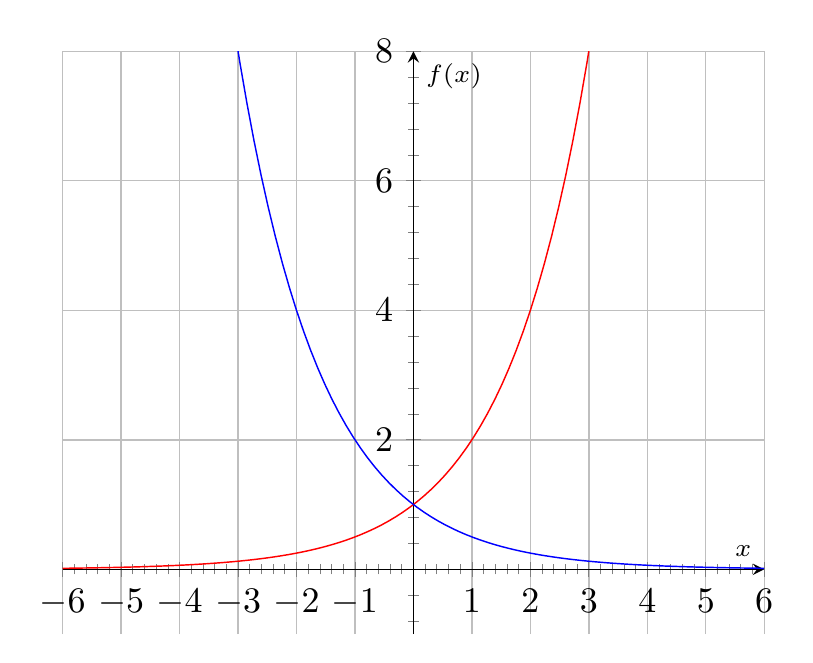
\begin{tikzpicture}[scale=1.3]
    \begin{axis}%
        [
            grid=major,
            xtick={-7,-6,...,7},
            minor x tick num=4, % 4 minor ticks => 5 subintervals
            xmin=-6,
            xmax=6,
            xlabel={\scriptsize $x$},
            axis x line=middle,
            ytick={-1,-5,...,7},
            minor y tick num=4,  % 4 minor ticks => 5 subintervals
            ymin=-1,
            ymax=8,
            ylabel={\scriptsize $f(x)$},
            axis y line=middle,
            no markers,
            samples=100,
            domain=-6:6,
        ]
        \addplot[red] (x,{2^x});
        \addplot[blue] (x,{2^-x});
    \end{axis}
\end{tikzpicture}
\break
\newpage
\subsection{Potenzfunktionen}

$y=a*x^n$ mit $a=1$


\hfill \break
\textcolor{red}{n positiv und gerade}
\begin{itemize}
    \item Definitionsmenge: $O = \mathbb{R}$
    \item Wertemenge: $W = \mathbb{R}_0^{+}$
    \item streng monoton fallend in: $\mathbb{R}_0^{-}$
    \item streng monoton steigend in: $\mathbb{R}_0^{+}$
    \item Alle Grapen gehen durch folgende Punkte: $P(-1|1),P(0|0),P(1|1)$
\end{itemize}

\hfill \break
\textcolor{green}{n positiv und ungerade}
\begin{itemize}
    \item Definitionsmenge: $O = \mathbb{R}$
    \item Wertemenge: $W = \mathbb{R}$
    \item streng monoton fallend in: --
    \item streng monoton steigend in: $\mathbb{R}$
    \item Alle Grapen gehen durch folgende Punkte: $P(-1|-1),P(0|0),P(1|1)$
\end{itemize}

\hfill \break
\textcolor{blue}{n negativ und gerade}
\begin{itemize}
    \item Definitionsmenge: $O = \mathbb{R}$ ohne $\{0\}$
    \item Wertemenge: $W = \mathbb{R}^{+}$
    \item streng monoton fallend in: $\mathbb{R}^{+}$
    \item streng monoton steigend in: $\mathbb{R}^{-}$
    \item Alle Grapen gehen durch folgende Punkte: $P(-1|1),P(1|1)$
    \item Asymptote: x und y Achsen $x=0$ $y=0$
\end{itemize}

\newpage
\textcolor{violet}{n negativ und gerade}
\begin{itemize}
    \item Definitionsmenge: $O = \mathbb{R}$ ohne $\{0\}$
    \item Wertemenge: $W = \mathbb{R}$ ohne $\{0\}$
    \item streng monoton fallend in: $\mathbb{R}$ ohne $\{0\}$
    \item streng monoton steigend in: --
    \item Alle Grapen gehen durch folgende Punkte: $P(-1|-1),P(1|1)$
    \item Asymptote: x und y Achsen $x=0$ $y=0$
\end{itemize}

\hfill \break
Graptische darstellung:
\hfill \break
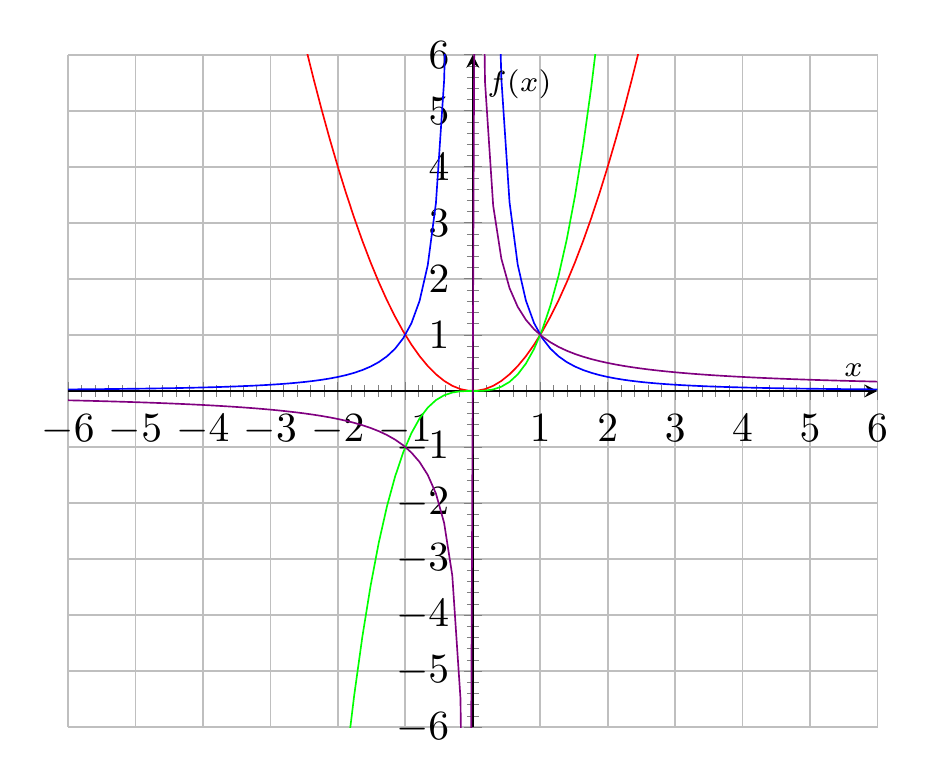
\begin{tikzpicture}[scale=1.5]
    \begin{axis}%
        [
            grid=major,
            xtick={-7,-6,...,7},
            minor x tick num=4, % 4 minor ticks => 5 subintervals
            xmin=-6,
            xmax=6,
            xlabel={\scriptsize $x$},
            axis x line=middle,
            ytick={-7,-6,...,7},
            minor y tick num=4,  % 4 minor ticks => 5 subintervals
            ymin=-6,
            ymax=6,
            ylabel={\scriptsize $f(x)$},
            axis y line=middle,
            no markers,
            samples=100,
            domain=-6:6,
        ]
        \addplot[red] (x,{1*x^2});
        \addplot[green] (x,{1*x^3});
        \addplot[blue] (x,{1*x^(-2)});
        \addplot[violet] (x,{1*x^(-1)});
    \end{axis}
\end{tikzpicture}
\break
\newpage
\subsection{Umkehr-Funktionen}

\hfill \break
\begin{itemize}
    \item Grapisch wird die Umkehrfunktionen durch das Spiegeln an der 1.Mediane ermittelt
    \item Rechnerisch wird die Umkehrfunktionen durch das Vertauschen von x und y ermittelt. zb.
          $y=10^x \rightarrow x=10^y \rightarrow y=Lg(x)$
\end{itemize}

\hfill \break
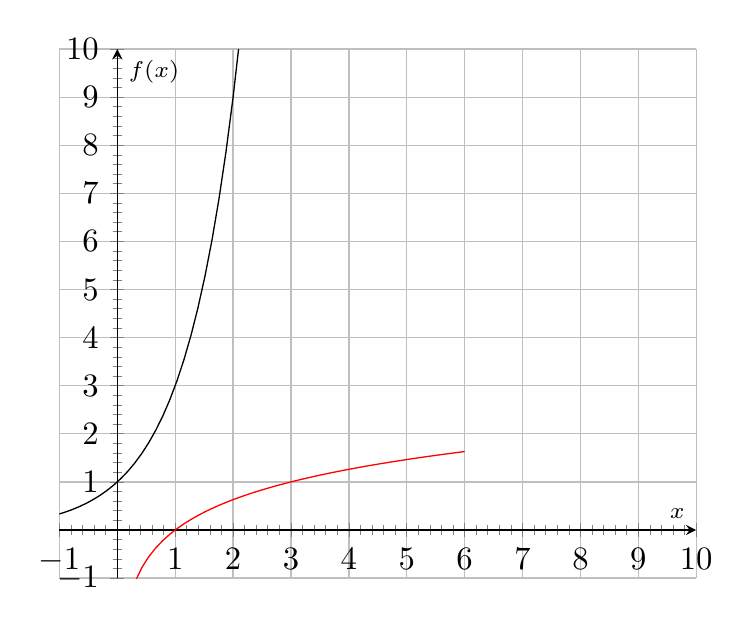
\begin{tikzpicture}[scale=1.18]
    \begin{axis}%
        [
            grid=major,
            xtick={-1,0,...,10},
            minor x tick num=4, % 4 minor ticks => 5 subintervals
            xmin=-1,
            xmax=10,
            xlabel={\scriptsize $x$},
            axis x line=middle,
            ytick={-1,0,...,10},
            minor y tick num=4,  % 4 minor ticks => 5 subintervals
            ymin=-1,
            ymax=10,
            ylabel={\scriptsize $f(x)$},
            axis y line=middle,
            no markers,
            samples=100,
            domain=-6:6
        ]
        \addplot[black] (x,{3^x});
        \addplot[red] (x,{ln(x)/ln(3)}); 
    \end{axis}
\end{tikzpicture}

\subsubsection{Graphen schneiden mit TR}

\hfill \break
Example:\\
\fboxrule=0.8pt \fcolorbox{black}{lightgray}{%
    \begin{tabular}[t]{@{}l@{}}
        $y = -x^3+8x-3$    \\
        $y = x^2-6x+9$     \\
        \\
        2nd calc intersect \\
        \\
        $S(1\vert4)$       \\
        $S(6\vert 9)$      \\
    \end{tabular}}\\
